%% Submissions for peer-review must enable line-numbering
%% using the lineno option in the \documentclass command.
%%
%% Preprints and camera-ready submissions do not need
%% line numbers, and should have this option removed.
%%
%% Please note that the line numbering option requires
%% version 1.1 or newer of the wlpeerj.cls file, and
%% the corresponding author info requires v1.2

\documentclass[fleqn,10pt,lineno]{wlpeerj} % for journal submissions
% \documentclass[fleqn,10pt]{wlpeerj} % for preprint submissions
\usepackage{graphicx}
\usepackage{listings}
\title{Counting Males and Females from Internet in Sociology. Damegender and GNU/Linux as Use Case}
\usepackage{url}

\author[1]{David Arroyo Menéndez}
\affil[1]{Universidad Rey Juan Carlos}
\author[2]{Jesús González Barahona}
\affil[2]{Universidad Rey Juan Carlos}
\author[3]{Gregorio Robles}
\affil[3]{Universidad Rey Juan Carlos}


\keywords{Gender gap, Gender detection tools, Software repositories}
\begin{abstract}
To achieve gender equality, first we need to measure gender in a
population to detect if gender gap exists. Damegender is a gender
detection tool that takes names as input returning the
gender~\cite{menendez2020damegender}.

The gender detection tools from the names are being used usually with
commercial APIs. But in recent years, many countries have released
data on the frequency and gender of names of their population with
Open Data Licenses. So, Damegender uses these datasets in an
industrial way and gives a new, original solution to classify gender
using names as input -- although we are using Machine Learning
algorithms to predict the gender for names that do not appear in the
datasets, such as nicknames or new names.

Damegender uses Perceval~\cite{duenas2018perceval} to count males and
females in a lot of Internet Communities (mailing lists, software
repositories, ...) In this paper we present how to use this tool in
sociology.
\end{abstract}

\begin{document}

\flushbottom
\maketitle
\thispagestyle{empty}

\section*{1. Introduction}
Any gender study takes into account previous studies with different
objectives and to collect data towards the objective proposed. The
gender detection tools from the names can be used when the objective
has been defined.

A gender detection tool from the name has a string as input, for
instance, Alicia and returns a gender (male or female, generally) with
a probability.

These tools has been used in global problems as to measure the gender
gap in science~\cite{holman2018gender} using sources as PubMed and
arXiv and counting males and females from author names. You can use
Damegender with global objectives or in Internet communities with
specific objectives.

In this paper, we are going to explain how to use Damegender (the
gender detection tool from common names developed by us) applied to
sociology with an use case: to measure males and females in a
GNU/Linux operating system.

\section*{2. MATERIAL AND METHODS}

\subsection*{Gender Inequality in the World}

Gender gap or gender inequality is the idea that men and women are not
equal and that gender affects an individual's living experience. These
differences arise from distinctions in biology, psychology, and
cultural norms. Some of these types of distinctions are empirically
grounded while others appear to be socially constructed. Studies show
the different lived experience of genders across many domains
including education, life expectancy, personality, interests, family
life, careers, and political affiliations. Gender inequality is
experienced differently across different cultures.\footnote{seen in
  https://wikipedia.org, 2020}.

The women is underrepresented in the labour world (among adults aged
from 25 to 54 has stagmated over the past 20 years, standing at 31
percentage points. The gender pay gap exists, too, so the women are
paid 16\% less than men. Share of women and men with an account at a
financial institution is 65\% of the total in women and 72\% of the
total in men. 31\% of young women aged 15 to 24 are not in education,
employment or training in 2020, more than double rate for young men
(14\%). Violence against women is 18\% of ever-partnered women aged 15
to 49 experienced sexual and/or physical violence by an intimate
partner in the previous 12 months.\footnote{https://www.unwomen.org}.

First, we can determine gender gap in several continents. From the
best score to the worst score. We can find: North America with the
best score, Europe and Central Asia, Latin America and the Caribbean,
Sub-Saharan Africa, Asia and the Pacific, and the worst score Middle
East and South Africa.~\cite{hausmann2012global}

\subsection*{Gender Gap in STEM}

In ~\cite{holman2018gender}, explains that the gap publishing in STEM
is especially large in authorship positions associated with seniority,
and prestigious journals have fewer women authors. Additionally, they
estimate that men are invited by journals to submit papers at
approximately double the rate of women. Wealthy countries, notably
Japan, Germany, and Switzerland, had fewer women authors than poorer
ones.

The Gender Shares of Total and STEM Jobs is 76\% men and 24\% women
compared with 52\% men and 48\% women in all jobs
~\cite{beede2011women}

We can find summarize six explanations~\cite{wang2017gender} for US
women’s underrepresentation in math-intensive STEM fields: (a)
cognitive ability, (b) relative cognitive strengths, (c) occupational
interests or preferences, (d) lifestyle values or work-family balance
preferences, (e) field-specific ability beliefs, and (f)
gender-related stereotypes and biases.

\subsection*{Philosophies about software, market, freedom and gender}

There are different philosophies developing software and we are
counting males and females in Internet, so the floor is the software
in this world. If we must analyze gender in a country the ideology is
changing in the place where you are. In the software world is the same
problem. So, we are giving the vocabulary and the philosophy for speak
about software and ideologies.

The propietary software is the most common idea for the common people,
operating systems such as Microsoft Windows or Mac OS. If you are
using software with propietary licenses, the source files will be
containing copyright notes such as:

\begin{verbatim}
# Copyright (C) 2020  David Arroyo Menéndez

# Author: David Arroyo Menéndez <davidam@@gmail.com>
# Maintainer: David Arroyo Menéndez <davidam@@gmail.com>

# All rights reserved}
\end{verbatim}

This idea is associated to big companies leading the market but any
people can use this philosophy. The criticism appears with Richard
Stallman about privacy and the lack of freedom to the academic people,
or hackers (people who knows read and write software and they do it
for his objectives or global objectives). I could to say the monopoly
is too strong with this license and the current social inertia and now
nobody can change the market, we need another licenses to preserve the
free market with an ethical strategy for startups and students.

Richard Stallman defines the Free Software with four freedoms: (0) to
run the program, (1) to study and change the program in source code
form, (2) to redistribute exact copies, and (3) to distribute modified
versions. ~\cite{stallman2002free}

This idea to build software as a social good and motivated by ethical
values. The solution is to apply the GPL license and to request to GNU
to include the software.

The copyright note in GNU would be similar to:

\begin{verbatim}
;; This software is free software: you can redistribute it and/or modify
;; it under the terms of the GNU General Public License as published by
;; the Free Software Foundation, either version 3 of the License, or
;; (at your option) any later version.

;; This software is distributed in the hope that it will be useful,
;; but WITHOUT ANY WARRANTY; without even the implied warranty of
;; MERCHANTABILITY or FITNESS FOR A PARTICULAR PURPOSE.  See the
;; GNU General Public License for more details.

;; You should have received a copy of the GNU General Public License
;; along with GNU Emacs.  If not, see <https://www.gnu.org/licenses/>.
\end{verbatim}

On opposition the Open Source movement believes in free licenses, but
they thinks that the software is business and they want to develop
Free Software by economy, so they prefer change the word Free Software
by Open Source claiming their philosophy.

They redefines the Free Software Definition by the Open Source
Definition~\cite{perens1999open}.

1. Free Redistribution

The license shall not restrict any party from selling or giving away
the software as a component of an aggregate software distribution
containing programs from several different sources. The license shall
not require a royalty or other fee for such sale.

2. Source Code

The program must include source code, and must allow distribution in
source code as well as compiled form. Where some form of a product is
not distributed with source code, there must be a well-publicized
means of obtaining the source code for no more than a reasonable
reproduction cost, preferably downloading via the Internet without
charge. The source code must be the preferred form in which a
programmer would modify the program. Deliberately obfuscated source
code is not allowed. Intermediate forms such as the output of a
preprocessor or translator are not allowed.

3. Derived Works

The license must allow modifications and derived works, and must allow
them to be distributed under the same terms as the license of the
original software.

4. Integrity of The Author's Source Code

The license may restrict source-code from being distributed in
modified form only if the license allows the distribution of "patch
files" with the source code for the purpose of modifying the program
at build time. The license must explicitly permit distribution of
software built from modified source code. The license may require
derived works to carry a different name or version number from the
original software.

5. No Discrimination Against Persons or Groups

The license must not discriminate against any person or group of
persons.

6. No Discrimination Against Fields of Endeavor

The license must not restrict anyone from making use of the program in
a specific field of endeavor. For example, it may not restrict the
program from being used in a business, or from being used for genetic
research.

7. Distribution of License

The rights attached to the program must apply to all to whom the
program is redistributed without the need for execution of an
additional license by those parties.

8. License Must Not Be Specific to a Product

The rights attached to the program must not depend on the program's
being part of a particular software distribution. If the program is
extracted from that distribution and used or distributed within the
terms of the program's license, all parties to whom the program is
redistributed should have the same rights as those that are granted in
conjunction with the original software distribution.

9. License Must Not Restrict Other Software

The license must not place restrictions on other software that is
distributed along with the licensed software. For example, the license
must not insist that all other programs distributed on the same medium
must be open-source software.

10. License Must Be Technology-Neutral

No provision of the license may be predicated on any individual
technology or style of interface.


In the point six, we find the conflict with the feminist theories due to
the possitive discrimination is a good idea to reach gender equity.

The GNU philosophy has the same problem explained on a different
way. Only the Free Software is a good idea, if the software is not Free
Software, then it's Propietary Software (the bad idea to avoid).

Generally, a worker in a company can extract ideas from GNU and Open
Source movements from the economical interest in a equlibrium with the
ideology.

\subsection*{Multiculturalism, Interculturalism}

The term multiculturalism has a range of meanings within the contexts
of sociology, of political philosophy, and of colloquial use. In
sociology and in everyday usage, it is a synonym for "ethnic
pluralism", with the two terms often used interchangeably, for
example, a cultural pluralism in which various ethnic groups
collaborate and enter into a dialogue with one another without having
to sacrifice their particular identities. It can describe a mixed
ethnic community area where multiple cultural traditions exist (such
as New York City or Trieste) or a single country within which they do
(such as Switzerland, Belgium or Russia). Groups associated with an
indigenous, aboriginal or autochthonous ethnic group and
settler-descended ethnic groups are often the focus.

In reference to sociology, multiculturalism is the end-state of either
a natural or artificial process (for example: legally-controlled
immigration) and occurs on either a large national scale or on a
smaller scale within a nation's communities. On a smaller scale this
can occur artificially when a jurisdiction is established or expanded
by amalgamating areas with two or more different cultures (e.g. French
Canada and English Canada). On a large scale, it can occur as a result
of either legal or illegal migration to and from different
jurisdictions around the world (for example, Anglo-Saxon settlement of
Britain by Angles, Saxons and Jutes in the 5th century or the
colonization of the Americas by Europeans, Africans and Asians since
the 16th century).

In reference to political science, multiculturalism can be defined as
a state's capacity to effectively and efficiently deal with cultural
plurality within its sovereign borders. Multiculturalism as a
political philosophy involves ideologies and policies which vary
widely. It has been described as a "salad bowl" and as a "cultural
mosaic", in contrast to a "melting pot". (Source: wikipedia, 2020)

Interculturalism refers to support for cross-cultural dialogue and
challenging self-segregation tendencies within cultures.
Interculturalism involves moving beyond mere passive acceptance of a
multicultural fact of multiple cultures effectively existing in a
society and instead promotes dialogue and interaction between
cultures.

Interculturalism has arisen in response to criticisms of existing
policies of multiculturalism, such as criticisms that such policies
had failed to create inclusion of different cultures within society,
but instead have divided society by legitimizing segregated separate
communities that have isolated themselves and accentuated their
specificity. It is based on the recognition of both differences and
similarities between cultures. It has addressed the risk of the
creation of absolute relativism within postmodernity and in
multiculturalism. (Source: wikipedia, 2020)

Aguado in ~\cite{odina1991educacion} propose these principles:

1. Promote the respect by all cultures together and condemn the
politics to change the culture of the people towards the culture
dominant. 

2. The intercultural education is relevant for any student, not only
for the foreigners and minorities.

3. The troubles created by the ethnic and cultural diversity of the
society has many solutions, there not an only magic solution. The
politics in education there are partials because we are in a global
society.

4. It's based in the perception about to accept cultures in contact,
it's near to the form of life of societies with a poor cultural
context instead of societies with more rich, more structure and high
social control.

5. We need develop a scheme of concepts with many cultures
demonstrating in the education that the knowledge is the common
property of all people.

So, interculturalism and multiculturalism are the same concept in many
uses, both recognize the cultural diversity in the contexts where
there are the diversity, but interculturalism is doing an emphasis in
the enrichment of all cultures respecting the diversity.

Damegender understands has an international and intercultural
perspective about guess the gender about the name in the sense that in
many countries are existing many different cultures determining names,
surnames with a gender. For example, in Spain are living 4 so
important cultures (no foreigners): Castillian (culture dominant),
Catalan, Basque and Galician.

These cultures has correlations with names and surnames.

\section*{3. RESULTS}

An operating system based on UNIX such as Ubuntu GNU/Linux or MacOS is
based on several parts we can divide Debian GNU/Linux in:

\begin{itemize}
	\item \texttt Debian is a distribution: the packaging to
          be downloaded from Internet or released on a CD or
          DVD. There are several distributions: Debian, Ubuntu, Suse,
          RedHat, ... We have chosen Debian as a case. These
          distributions mentioned are using GNU and Linux.
	\item \texttt Linux is the kernel: the part that is
          communicating with the hardware
	\item \texttt GNU is a project to create free operating
          system, many software such as editors, desktop, commands
          console, compilers, ... has been developed by this project.
	\item \texttt There are more software created by another
          projects in an operating system such as X Window System. But
          GNU/Linux is a good verbal agreement recognizying efforts.
\end{itemize}

This section is divided counting males and females in Debian, GNU and
Linux.

We have reached the csv files from different ways to know the names
about the people in these communities.

When this article was being wrote in the Debian community all members
must be collaborating with a gpg key, so we can count males and females
from the keyring. The keyring was imported with gpg commands and later
was dumped the keyring in a csv file.

In the moment to write this paper
GNU\footnote{https://www.gnu.org/people/} and
Linux\footnote{https://www.kernel.org/doc/html/latest/process/maintainers.html}
has websites with the people collaborating in these projects. So,
making webscraping scripts we have downloaded the people and processed
the people to csv files

Damengender is set of datasets and software related developed in
Python~\cite{van2011python}. We have developed csv2gender, a software
with a csv file as input and returns the result of males, females and
unknows and/or deploying a statistics graph.

To make easy to reproduce the experiment we are pasting the commands
used with the version 0.3.4 of damegender.

\begin{verbatim}
python3 csv2gender.py files/gnu-maintainers.csv
 --first_name_position=0 --title="GNU maintainers grouped by gender"
 --dataset="inter" --outcsv="files/gnu-maintainers.gender.csv"
 --outimg="files/gnu-maintainers.gender.png" --noshow
 --delete_duplicated

python3 csv2gender.py files/linux-maintainers.csv
 --first_name_position=0 --title="Linux maintaners grouped by gender"
 --dataset="inter" --outcsv="files/linux-maintainers.gender.csv"
 --outimg="files/linux-maintainers.gender.png" --noshow
 --delete_duplicated

python3 csv2gender.py files/debian-maintainers-gpg-2020-04-01.csv
 --first_name_position=0 --title="Debian maintaners grouped by gender"
 --dataset="inter" --outcsv="files/debian-maintainers.gender.csv"
 --outimg="files/debian-maintainers.gender.png" --noshow
 --delete_duplicated
\end{verbatim}

The inter dataset was created merging several open datasets downloaded
from official statistics sites from different nations: Austria,
Australia, Belgium, Canada, Germany, Denmark, Spain, Finland, Ireland,
Iceland, Mexico, New Zealand, Portugal, Slovenia, United States of
America, Uruguay and France. That's a good representation of the
Western World and the Free Software world is populating this world's
area~\cite{gonzalez2008geographic}.

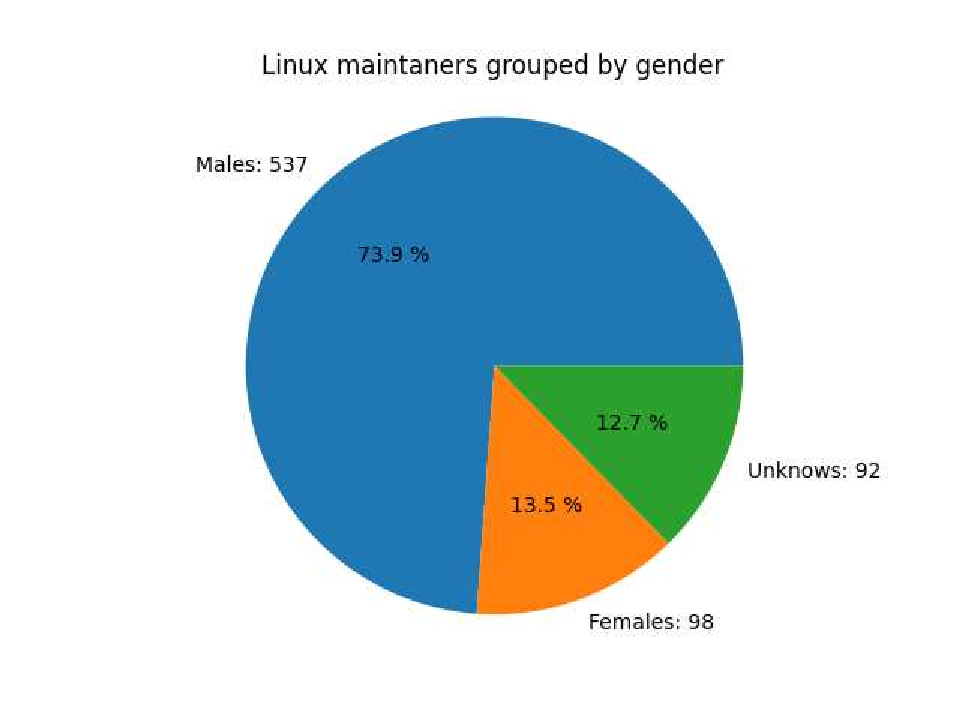
\includegraphics[width=0.8\textwidth]{images/linux-maintainers.gender.pdf}

Linux divides the developers in 537 males (73.9\%), 98 females
(13.5\%) and 92 unknows (12.7\%). The number of unknows is due to
different reasons, but it's so common in Linux that the developer is a
company and not a name of a person.

GNU divides the developers in 164 males (89.6\%), 12 females (6.6\%)
and 7 unknows (3.8\%)

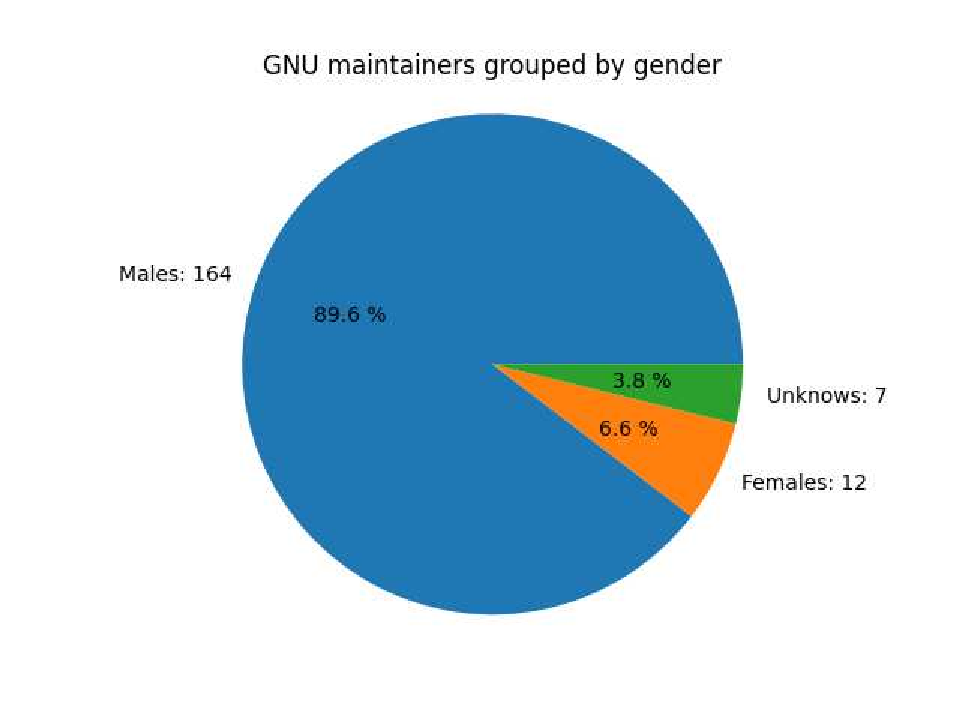
\includegraphics[width=0.8\textwidth]{images/gnu-maintainers.gender.pdf}

The GNU people has a number lowest in females, they are the founder of
the Free Software philosophy, the Debian principles and the Open
Source philosophy was invented later influenced by GNU with very
similar practical decisions (for example: deciding licenses for the
software). Richard Stallman returned to be president recently
apologizing by his personal behaviour with the
females.\footnote{https://www.fsf.org/news/rms-addresses-the-free-software-community}

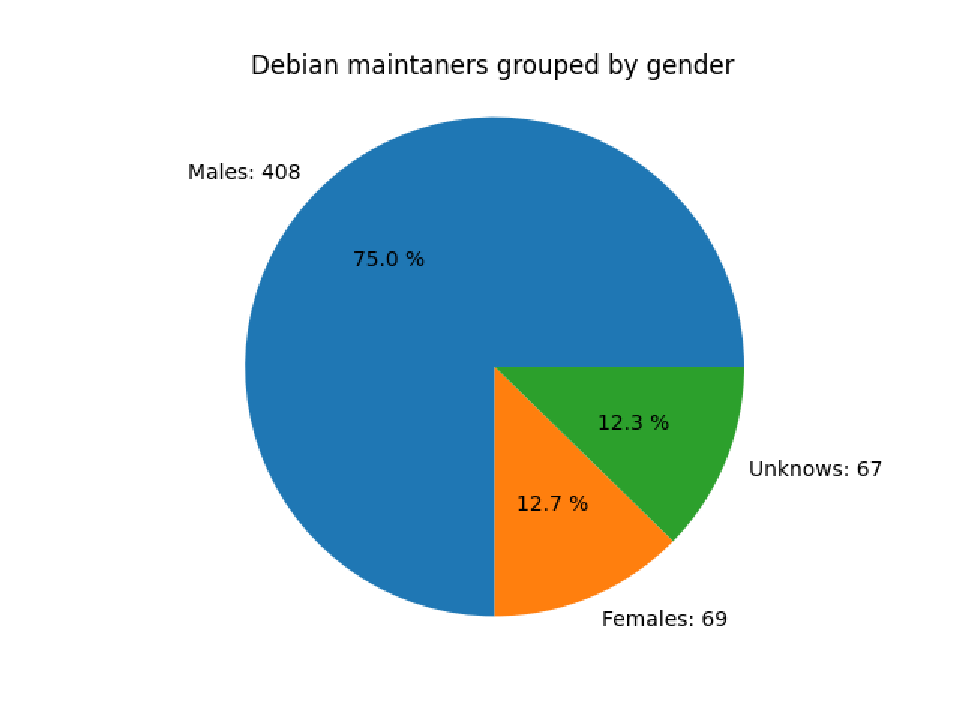
\includegraphics[width=0.8\textwidth]{images/debian-maintainers.gender.pdf}

Debian is a distribution, the project who makes the CD/DVD and the
software ready to be downloaded from Internet with the
dependencies. There are many distributions, such as, Ubuntu or RedHat
so it is not representative, but it's interesting to understand that
the numbers are similar in Debian dividing the developers in 408 males
(75\%), 69 females (12.7\%) and 67 unknows (12.3\%).


\section*{4. DISCUSSION}

The context of the operating systems is not feminist by different
reasons. In the Free Software world there are many males developing
the software. But in another Operating Systems there are another
problems about the male domination, for example, Microsoft created the
richest man in the world for many
years.\footnote{https://www.forbes.com/profile/bill-gates/}

Apple was classified as the most valuable company in the world in
2020.\footnote{https://www.forbes.com.mx/mercados-apple-empresa-mas-valiosa-del-mundo/}

By intersectionality, to create companies more powerful than some
states is bad for the democracy and the social change towards the
gender equity many times only funded by democracy values.

The Free Operating Systems is pressuring to the propietary operating
systems such as Windows or MacOS to change the philosophy about
licensing. So the gender gap dicussion in operating systems is a world
dominated by economical pressures of several companies where the
scientific population is closed to free software values due to they
implement the Free Software freedoms every day in their positions and
business in some way. On another hand, the powerful companies is
dominating the market about domestic users as monopolies against the
free software solutions funded by academical interests in the begining
and now by another companies such as Oracle or Google who is
investing on these markets with clever solutions such as Android or
MySQL with ideas for dominate these markets, too.

So, the ethical discussion about the free market is real in the
context of operating systems, although a software community can be
dominated by a strong company with investments.

The gender equity is the objective five in United Nations about
sustainable
development.\footnote{https://www.un.org/sustainabledevelopment/gender-equality/}

A good business must be living in harmony
with the values of the society, although earning money from many
points. So, the current situation in GNU/Linux must be fixed until the
average in STEM or TIC because many times are being compared with it,
improving the marketing about values that's using yet.

\section*{5. CONCLUSIONS}

The violence against the women sometimes is the structure of the
society and the software industry is a piece of the society. We need
defines terms and philosophies speaking about gender in the software
industry (intersectionality, feminism, ecofeminism, open source, free
software, interculturalism, ... ) has been defined to set words in the
contexts.

GNU/Linux is the option with a total penetration of market in
supercomputers, high penetration in servers and mobiles (Android is
using Linux) and low in desktops

The gender gap exists in STEM, but it's bigger in GNU/Linux with a
rate about women varying from 6\% until 13\%. We can to count the
gender gap in different contexts with Open Datasets and to measure and
to evaluate evolution by years if there are people with this
objective, skills and time to invest on it.

So, the marketing about ethical values in GNU/Linux could be improved
deleting the gender gap due to it's bigger than the average in STEM.

\section*{6. BIBLIOGRAPHICAL REFERENCES.}

\bibliography{sociotecno.bib}

\end{document}
